
\begin{center}
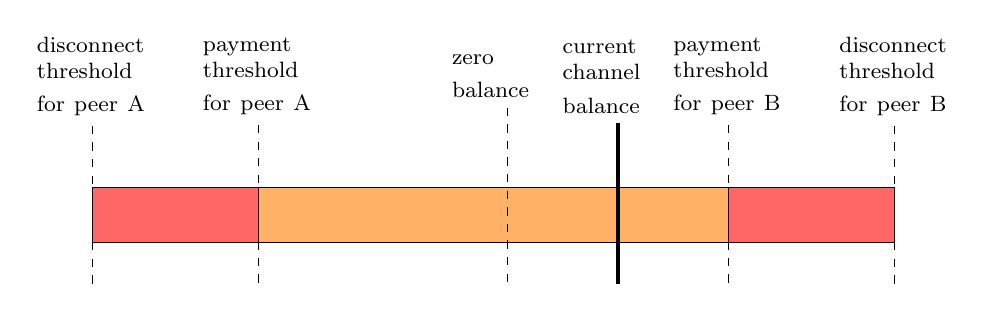
\begin{tikzpicture}
\node (middle)[draw, rectangle, fill=orange!60, minimum height=2em, minimum width=18em]{};
\node (leftred) [draw, rectangle, fill=red!60, minimum height=2em, minimum width=6em, node distance=12em,left of=middle]{};
\node (rightred)[draw, rectangle, fill=red!60, minimum height=2em, minimum width=6em, node distance=11em,right of=middle]{};
\node (zero) [above of=middle,node distance=5em, text width=4em, align=left] {\footnotesize zero\\ balance};
\node (zerod) [below of=middle] {};
\draw [dashed](zero)--(zerod);
\node (rtol) [node distance=8em,right of=zero,text width=4em, align=left] {\footnotesize payment\\threshold\\for peer B};
\node (rtold) [node distance=8em,right of=zerod] {};
\node (ltol) [node distance=9em,left of=zero,text width=4em, align=left] {\footnotesize payment\\threshold\\for peer A};
\node (ltold) [node distance=9em,left of=zerod] {};
\node (rdis) [node distance=14em, right of=zero,text width=4em, align=left] {\footnotesize disconnect\\threshold\\for peer B};
\node (rdisd) [node distance=14em,right of=zerod] {};
\node (ldis) [node distance=15em, left of=zero,text width=4em, align=left] {\footnotesize disconnect\\threshold\\for peer A};
\node (ldisd) [node distance=15em,left of=zerod] {};
\node (rbal) [node distance=4em,right of=zero,text width=4em, align=left] {\footnotesize current\\channel\\balance};
\node (rbald) [node distance=4em,right of=zerod] {};

\draw [dashed](rtol)--(rtold);
\draw [dashed](ltol)--(ltold);
\draw [dashed](rdis)--(rdisd);
\draw [dashed](ldis)--(ldisd);
\draw [very thick](rbal)--(rbald);
\end{tikzpicture}
\end{center}